\chapter{$C^{++}$-basics \label{chapBasicCPP}}

\pagenumbering{arabic}

%------------------------------------------------------------------------

\section{Structure of a simple program}

Similar to C, any C++ program has at least one function, the function
\verb+main+. This function is generally referred to as the main program.
The body of any function is enclosed within curly brackets ($\{ \dots \}$)
each statement is terminated by a semicolon.
The curly brackets perform the function of the \verb+begin+ \dots \verb+end+
block in other languages like, for example, Pascal.

Lets have a look at the C++ version of the traditional {\it ``Hello World''} program:

\noindent {\small \input{BasicCPP/Programs/HelloWorld.cpp}}

\noindent
The first line includes the header file input/output stream class library. Later we
shall see that this is a hierarchy of classes for accessing input and output devices.
Header files are used to inform the user of the constants, variables, functions and
classes defined in the accompanying CPP (implementation) file. You can include
standard libraries supplied with your compiler, third party libraries acquired
from some vendor (e.g. a database library) or libraries you wrote yourself.

The latest ANSI  C+ standard packagess the standard library elements in the
standard namespace. Name spaces will be discussed in detail in chapter
\ref{chapNameSpaces}. For now it is sufficient to  state that name spaces
are C++'s support for packaging.

Next we define the \verb+main+ function of the program. Every C++ program
must have at least one function (and hence one non-object oriented element).
Its name must be \verb+main+. The \verb+void+ specifies that the function \verb+main+
has no return value. Functions which do not return a value are often called procedures.
The empty bracket after \verb+main+ specify that \verb+main+
takes no arguments. Later we shall show how we can give arguments to \verb+main+
in order to handle command line parameters.

Each function has a body. The body is enclosed within curly brackets. Our function has
only one statement. Statements in C++ are terminated by a semicolon. In this statement
we simply send the string \verb+"Hello World"+ to the standard output device \verb+cout+
which usually is the terminal. Data for output are passed to \verb+cout+ with the output
operator \verb+<<+. To be able to fully understand stream input/output one has to
understand classes and operator overloading. This will be covered in detail in the
following chapters. At this stage we shall simply use output streams as illustrated in
the {\it ``Hello World''} application.

The \verb+endl+ stream manipulator starts a new line and flushes the stream. It is very common
for C++ programmers to use the end-of-line character '/n' instead, but this does not flush
the stream and if the program aborts, some of the stream output might be lost.

%-------------------------------------------------------------------------------

\subsection{Compiling and running the program}

The process for compiling and running the program depends on both, the
compiler used and thhe target platform. We shall use the GNU C++ compiler.
In that case we can compile thhe application via

{\small \begin{verbatim}
g++ -Wall -ansi HelloWorld.cpp -o HelloWorld
\end{verbatim}}

This will generate an executable file which is called \verb+HelloWorld+
on Unix-type operating systems (e.g.\ {\em Linux}) and \verb+HelloWorld.exe+
on {\em Windows}.

On {\em Unix/Linux} we run the application from thhe directory in  which
the executable is stored via
{\small \begin{verbatim}
./HelloWorld<ENTER>
\end{verbatim}}

On {\em Windows} you would use
{\small \begin{verbatim}
HelloWorld<ENTER>
\end{verbatim}}
instead.
%-------------------------------------------------------------------------------

\subsection{Adding comments to your code}

Informative, unambiguous commenting and consistent indentation can make the task of
understanding code (even your own code when you come back to it after a while)
much more understandable. You must, however, take care to maintain your comments
together with your code. Otherwise you can easily end up with comments which are
ambiguous or even simply wrong. Such comments are worse than no comments at all.

There are two ways in which you can add comments to your C++ code. Both are
illustrated in the commented version of the {\it``Hello World''} application given
below:

\noindent {\small \input{BasicCPP/Programs/HelloWorld.cpp}}

\noindent
You can use the \verb+/* ... */+ comment to insert a comment which possibly spans
over several lines. For example, at the top of the file we give  the name of the
file in which the program is stored and then a description of what the program does.

Alternativerly you use a double-slash (\verb+//+) to specify that the remainder of that
line should be treated by as a comment. For example, after \verb+#include <iostream.h>+
precompiler directive we explain why we need the library.

Do not comment statements which are obvious from the code anyway. For example
adding a comment after the \verb+include+ statement that we are including the
\verb+iostream+ library gives us no further information and just increases the
amount of text the reader has to read and the amount of work involved when
changing the code (since we have to update the comments too).

%===================================================================

\section{Declarations}

There are 5 basic data types\index{basic data types} and 5 qualifiers
in $C^{++}$. These are shown in figure \ref{figPrimitives}.

%\begin{latexonly}
  \begin{figure}[htb]
    \begin{center}  
      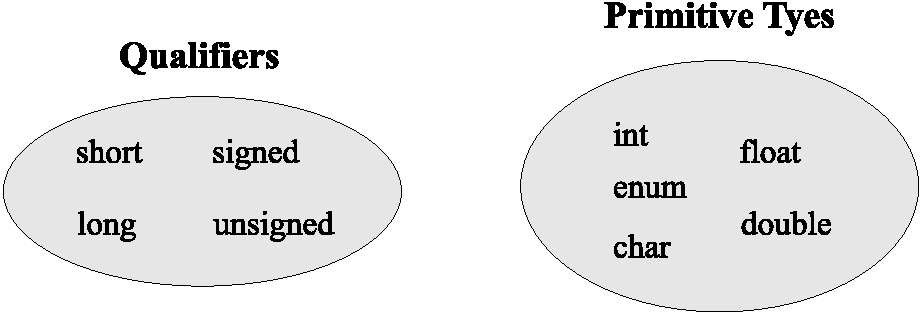
\includegraphics{BasicCPP/Figures/Primitives.pdf}
    \end{center}  
    \caption{The qualifiers can be combined with the primitive types to 
             specify new primitive types.
             \label{figPrimitives}} 
  \end{figure}
%\end{latexonly}  

%\begin{htmlonly}
%  \begin{rawhtml}
%    <center>
%      <img src="BasicCPP/Figures/Primitives.gif">
%    </center>
%    <br>
%%    <center>
%        The qualifiers can be combined with the primitive types to 
%             specify new primitive types.
%    </center>
%  \end{rawhtml}  
%  \begin{figure}\label{figPrimitives}\end{figure}
%  \vspace{5mm}
%\end{htmlonly}  

The data type \verb+char+ is a single byte, big enough to
hold a single character. The qualifiers and the basic types can be combined.
For example, one can have
{\small \begin{verbatim}
unsigned int i = 120, j;

int k;

long double  x, y, z = 21.2345677;

enum vehicle {bicycle, car, bus, truck, unknown=99} verhicle1, verhicle2;
\end{verbatim}}

\noindent
Here \verb+i+ and \verb+j+ are unsigned integer variables and \verb+i+
is initialized to $120$. \verb+k+ is an integer variable (per default
\verb+ unsigned short+), and \verb+x, y+ and \verb+z+ are long double
precision variables (on the IBM-PC usually 80 bits long ranging between
$3.4 \times 10^{-4932}$ to $1.1 \times^{+4932}$ with an accuracy of
about 21 decimal digits). The size of any data type can be obtained
with the $C^{++}$-function \verb+sizeof(datatype)+. \index{\verb+sizeof+}

\verb+verhicle1+ and \verb+verhicle2+ are enumeration
variables \index{enumeration type} which can only take one of the values \verb+bicycle+,
\verb+car+, \verb+bus+ and \verb+truck+ or unknown. Enumeration types
\index{\verb+enum+, enumeration type} are really named integer constants. In the above
example the compiler assigns \verb+bicycle=0+,
\verb+car=1+, \verb+bus=2+, \verb+truck=3+ and \verb+unknown=99+.
Note that \verb+vehicle+ is a new data type and variables of that type
can be declared like any other variable type:
{\small \begin{verbatim}
vehicle verhicle3;
\end{verbatim}}
\noindent
Variables of any data type can be declared constant:
{\small \begin{verbatim}
const long double  pi = 3.1415926535897932;
\end{verbatim}}
\noindent
If a certain variable should always remain constant it should be declared so. This
enables the compiler to report any violation of the constantness and thus enhances
program integrity.

%-------------------------------------------------------------------------

\subsection{Type-casting}

\subsubsection{Implicit type-casting}

The fundamental data types can be mixed freely in assignments and expressions.
In arithmetic  expressions the types are converted as to loose as little information
as possible. If either of the operands has higher resolution, then the other operand
is automatically converted to the higher resolution. For example adding a
\verb+float+ and a \verb+long double+ causes the \verb+float+ to be converted
to a \verb+long double+ and the result is a \verb+long double+. Similarly, integral
data types are promoted to the type with the largest range and if mixing integral
and floating point data types then the integral data type is promoted to a floating
point. Hence, adding an \verb+int+ to a \verb+double+ causes the \verb+int+ to be
converted to a \verb+double+ and the result is a \verb+double+.

We can also assign any fundamental data type to any other fundamental data type.
If we assign a \verb+float+ to a \verb+double+ the extra resolution is simply padded
by zeros. The other way around we will, of course, necessarily loose resolution (the
least significant digits will be truncated).

Similarly, assigning an integral data type to a floating point data type is no problem.
The decimal digits are simply set to zero. The other way around results in the
truncation of the decimal digits.

%----------------------------------------------------------------------------

\subsubsection{Explicit type casting}
In some cases it is necessary to type-cast explicitly. For example
{\small \begin{verbatim}
double x = 2/3;
\end{verbatim}}
\noindent
sets \verb+x+ to zero since division has presedence over assignment and the two data
types participating in the division are both integral data types -- hence integer division
is used, yielding zero. In this case one would explicitely type-cast one of the integers
to a \verb+double+:
{\small \begin{verbatim}
double x = (double)x/3;
\end{verbatim}}
\noindent
C++ supports two notations for type-casting. The traditional $C$-cast shown above and
the functional notation
{\small \begin{verbatim}
double x = double(x)/3;
\end{verbatim}}
The $C$ type-casting notation has the advantage that it also works with non-simple
type names:
{\small \begin{verbatim}
long double x = long double(x)/3;   // compiler generates error

long double x = (long double)x/3;   // no problem
\end{verbatim}}
Similarly, pointers (see later in this chapter) have to type-cast with the $C$-cast.

In later chapters we shall show how you can support implicit and explicit type-casting
for your own data types (classes).

%-------------------------------------------------------------------------

\subsubsection{Identifier names}

The name of an identifier (e.g.\ a variable, a constant or a function) consists
of a sequence of letters, digits and underscore-characters. The first character
may not be a digit. C++ does not impose a limit on the name-length. Some
compiler may however impose such a limit. A C++ keyword may of course not
be used for an identifier name.

Examples of legal identifier names are
{\small \begin{verbatim}
street_name    x    X    _X    x_    OS_2
\end{verbatim}}
\noindent
On the other hand, the following names are not legal identifier names:
{\small \begin{verbatim}
street-name    1x    OS/2    $system    first.name
\end{verbatim}}

%---------------------------------------------------------------------------------------

\subsubsection{Reference types}

Reference types allow us to access the same object by different names -- i.e.\ a reference
is an alias for an object of a specified type. Consider the following code snippet:
{\small \begin{verbatim}
int  i = 3;
int& ir = i;   // Reference to the variable i
ir = 5;
cout << i;     // Prints 5 on the screen
\end{verbatim}}
\noindent
After assigning the reference variable \verb+ir+ to \verb+i+, bot \verb+i+ and
\verb+ir+ use the same memory location. Changing the one will change the other.

We can make the reference as such a constant via \verb+const int& ir = i;+. This
will fix \verb+ir+ such that it will always use the same memory area as the
object \verb+i+. Alternatively, we can have a reference to a constant object:
{\small \begin{verbatim}
const double pi = 3.1415926;
double& ref = pi;   // Reference to the variable i
\end{verbatim}}
\noindent
Now, as long as \verb+ref+ is a reference to \verb+pi+, neither \verb+pi+ nor
\verb+ref+ may be changed. We can of course reassign the reference variable
to be an alias for another \verb+double+ object via, for example, \verb+ref = x;+.
Finally we can have a constant reference point to a constant object as in the
following example
{\small \begin{verbatim}
const double pi = 3.1415926;
const double& pi2 = pi;   // Reference to the variable i
\end{verbatim}}

We shall see that reference types are closely related to pointer types. Furthermore,
reference variables are very important for function arguments
(see section \ref{secPassRef}).

%-------------------------------------------------------------------------

\subsection{The scope and lifespan of variables}

In C++ blocks are delimited by curly brackets. For example the function body
is a block delimited by curly brackets. Within the function body we can declare
further blocks (nested blocks). The scope of a variable is
bounded by the block in which it is defined. Consider, for example, the following
program listing:

\noindent {\small \input{BasicCPP/Programs/ScopeTest.cpp}}

\noindent
Here \verb+version+ is a global floating point constant which has the scope of
the file, i.e.\  it can be used anywhere in the file. Similarly, we define a global
variable \verb+y+. In the function \verb+f+ we declare a local variable \verb+y+
which hides the global \verb+y+. The scope of this variable is within curly brackets
-- hence within the body of the function.

In the main program we use \verb+cout+ to write to the terminal and \verb+cin+ to
read in the value of \verb+a+ from the keyboard. The assignment statement
\verb+y = f(a)+ assigns the global \verb+y+ to the result of the function call.

We then check whether \verb+y+ is greater then \verb+5+ and if this is the case
we perform a collection of statements enclosed in a block (within curly brackets).
The \verb+if+ statement will be discussed in detail later in this chapter. Within the
block we declare a local variable, \verb+y+, which hides the global \verb+y+. The
scope of this variable is limited to the \verb+if+-block.

Generally it is a good idea to define variables as close to the point
where they are used as is possible. This makes maintenance usually a lot easier.
The use of global variables should be minimized. In fact, it is a good idea to
define your variables such that they have the minimum required scope. It is
even possible to restrict the scope of a variable to a subset of sequential
statements by enclosing this subset of statements simply within curly brackets.

%----------------------------------------------------------------------

\subsubsection{Lifespan of static variables}

Except for the case where you declare a variable as \verb+static+, it's life-time
is the same as its scope. For example, in the previous listing, the
variable \verb+y+, whose scope is the \verb+if+-block, is created and initialized
with the statement \verb+double y = a*a-a;+ and is destroyed at the when
the execution thread leaves the \verb+if+-block.

A \verb+static+ variable has the life-time of the program, i.e.\
it is created when the program is started and destroyed only when the program
terminates. They are initialized the first time the execution thread passes through
the declaration.

For example, say you want to monitor the number of times a certain function
\verb+f+ has been called. You can define a static local variable \verb+ncalls+
as follows:
{\small \begin{verbatim}
double f(const double x)
{
  static int ncalls = 0;

  ++ncalls;
  cout << "f has been called " << ncalls << " times." << endl;

  return x*x;
}
\end{verbatim}}
\noindent
Here \verb+ncalls+ is initialized to zero the first time the function is called.
Then \verb+ncalls+ is incremented and its value is printed onto the terminal.
The next time \verb+f+ is called, the function remembers the value of
\verb+ncalls+ from its previous run, increments it and prints out the correct
no of function calls.

%-------------------------------------------------------------------------

\section{$C^{++}$ operators}

Table \ref{basiccppCppops} shows a summary of $C^{++}$ operators
\index{operators}
\index{operators!precedence} in order of decreasing precedence. Hence
\verb& u = x + y % z; & evaluates first the remainder of $\frac{y}{z}$,
then adds this to \verb+x+ and then assigns the result to \verb+u+
(note that \verb+10%4+ returns \verb+2+).


\begin{table}[hbt]
 \begin{center}
 \begin{footnotesize}
  \begin{tabular}{|lll|}
    \hline
    Operator & operator name & example \\
    \hline \hline
    \verb+::+ & scope resolution & {\it class\_name}\verb+::+{\it member} \\
    \verb+::+ & global           & \verb+::+{\it name} \\
    \hline
    \verb+.+  & member selection & {\it object}\verb+.+{\it name} \\
    \verb+->+ & member selection & {\it pointer}\verb+->+{\it member} \\
    \verb+[]+ & subscription     & {\it pointer}\verb+[+{\it expr}\verb+]+ \\
    \verb+()+ & function call    & {\it expr}\verb+(+{\it expr\_list}\verb+)+ \\
    \verb+()+ & value construction & {\it type}\verb+(+{\it expr\_list}\verb+)+ \\
    \verb+sizeof+ & size of object & \verb+sizeof+ {\it expr} \\
    \verb+sizeof+ & size of type   & \verb+sizeof(+{\it type}\verb+}+ \\
    \hline
    \verb&++& & post or pre increment     & {\it lvalue}\verb&++& or \verb&++&{\it lvalue} \\
    \verb+--+ & post or pre decrement     & {\it lvalue}\verb+--+ or \verb+--+ {\it lvalue} \\
    \verb+~+  & complement         & \verb+~+{\it expr} \\
    \verb+!+  & not                & \verb+!+{\it expr} \\
    \verb++ , -+  & unary plus and minus  & \verb+-+{\it expr} and \verb&+&{\it expr} \\
    \verb+&+  & address of         & \verb+&+{\it lvalue} \\
    \verb+*+  & dereferencing      & \verb+*+{\it expr} \\
    \verb+new+ & create (allocate memory) & \verb+new+ {\it type} \\
    \verb+delete+ & deallocate pointer memory  & \verb+delete+ {\it pointer} \\
    \verb+delete[]+ & free array memory & \verb+delete[]+ {\it pointer} \\
    \verb+()+ & cast (type conversion) & \verb+(+{\it type}\verb+)+ {\it expr} \\
    \hline
    \verb+.*+ & member section & {\it object}\verb+.*+{\it pointer-to-member} \\
    \verb+->*+ & member section & {\it pointer}\verb+->*+{\it pointer-to-member} \\
    \hline
    \verb& * , / , % & & multiply, divide, modulo (remainder)
                         & {\it expr} \verb+/+ {\it expr} \\
    \hline
    \verb&+ , -& & add, subtract & {\it expr} \verb&+& {\it expr} \\
    \hline
    \verb+<< , >>+ & shift left , shift right
                   & {\it expr} \verb+<<+ {\it expr} \\
    \hline
    \verb+< , <= , > , >=+ & relational operators
                & {\it expr} \verb+<+ {\it expr} \\
    \hline
    \verb+==+ & equal & {\it expr} \verb+==+ {\it expr} \\
    \verb+!=+ & not equal & {\it expr} \verb+!=+ {\it expr} \\
    \hline
    \verb+&+ & bitwise AND & {\it expr} \verb+&+ {\it expr} \\
    \hline
    \verb+^+ & bitwise exclusive OR & {\it expr} \verb+^+ {\it expr} \\
    \hline
    \verb+|+ & bitwise inclusive OR & {\it expr} \verb+|+ {\it expr} \\
    \hline
    \verb+&&+ & logical AND & {\it expr} \verb+&&+ {\it expr} \\
    \hline
    \verb+||+ & logical inclusive OR & {\it expr} \verb+||+ {\it expr} \\
    \hline
    \verb+? :+ & conditional expression & {\it expr} \verb+?+ {\it expr}
                            \verb+:+ {\it expr} \\
    \hline
    \verb+=+ & simple assignment & {\it lvalue} \verb+=+ {\it expr} \\
    \verb+*= , /= , += , -=+ & multiply and assign, \dots
                                 & {\it lvalue} \verb+*=+ {\it expr} \\
    \verb+<<= , >>=+ & shift left (right) and assign & {\it lvalue} \verb+<<=+ {\it expr} \\
    \verb+&= , |= , ^=+ & AND (OR, XOR) and assign & {\it lvalue} \verb+&=+ {\it expr} \\
    \hline
    \verb+throw+ & throw exception & \verb+throw+ {\it expr} \\
    \hline
    \verb+,+ & comma (sequencing) & {\it expr} \verb+,+ {\it expr} \\
    \hline
   \end{tabular}
   \end{footnotesize}
 \end{center}
 \caption{$C^{++}$ operators in order of decreasing precedence. Each
           box holds operators of the same level of precedence.
                \label{basiccppCppops}}
\end{table}

The use of these operators will be illustrated with example programs
throughout this text.

All operators can be overloaded \index{operators!overloading} (see
discussion on operator overloading later in the text) except for
{\small \begin{verbatim}
.    .*    ::    ?:
\end{verbatim}}
\noindent
When overloading operators, one should bare in mind that the order of precedence
and the syntax remains the same as that for the built-in data types.

\clearpage
%------------------------------------------------------------------------

\section{Control statements}
Control statements control the program flow. For example,
selection statements such as \verb+if ... else+  and
\verb+switch+ use certain criteria to select a course
of action within a program. Iterative control statements (like
\verb+for+, \verb+while ... do+, \verb+do ... while+ on
the other hand see to it that under certain conditions control
is passed from the last statement in a block to the first statement.

\subsection{Selection statements}

\subsubsection{The if-statement}

The following examples illustrate the \verb+if+ statement:
{\small\begin{verbatim}
int isPositive (const int x)
{
  if (x>=0) return 1;
  return 0;
}
\end{verbatim}}
\noindent
The condition is defined as {\bf false} if the argument is equal to zero
and {\bf true} otherwise. The else statement is similar to that of other
programming languages:
{\small\begin{verbatim}
void isZero (const double x)
{
  if (x)
    cout << "Argument is non-zero." << endl;
  else
   cout << "Argument is zero" << endl;
}
\end{verbatim}}
\noindent
The condition \verb+if (x)+ is equivalent to the condition \verb+if (x==0)+.
Note the difference between the ``is equal'' operator \verb+==+ and the
assignment operator \verb+=+.

Instead of executing a single statement conditionally, we can also execute a
block of statements conditionally:
{\small \begin{verbatim}
if ((x>0 && x*x<2) || (x==-1))
  {
    cout << "case 1: x = " << x << endl;
    x *= 3;
  }
else
 {
    cout << "case 2: x = " << x << endl;
    x /= 3;
 }
\end{verbatim}}
\noindent
Note that multiplication takes presedence over the relational operator \verb+<+
and that the relational operators take presedence over the logical and operator
\verb+&&+.

\subsubsection{The switch-statement}

One can nest \verb+if ... else+ statements to test for a number of conditions. In
cases where the conditions are integral constants, it is, however, more convenient
to use the \verb+switch+ statement (the equivalent of \verb+case+ statement of
Modula-2 or Ada).
{\small \begin{verbatim}
char c;  cin >> c;

switch(c)
{
  case 'a':  cout << "case a" << endl;
  case 'b':  cout << "case b" << endl;  break;
  case 'c':  cout << "case c" << endl;  break;
  default:  cout << "default code." << endl;
}
\end{verbatim}}
\noindent
The switch statement compares a variable of an integral type with an integral
constant defined at the \verb+case+ labels. Execution jumps to the first match found
and will continue sequentially. The case statements act like labeled statements.
Hence if the user presses the key \verb+'a'+, the output will be
{\small \begin{verbatim}
case a
case b
\end{verbatim}}
\noindent
Execution continues to the next statement (another \verb+case+ statement) until
a \verb+break+ is reached. The \verb+break+ statement can be used only in iteration
statements and in \verb+switch+ statements. In the case of the \verb+switch+ statement
it causes execution to jump out of the \verb+switch+ block. In the case of iteration
statements it causes execution to jump out of the innermost iterative loop.

If the user presses key 'b', or 'c' the screen output will be \verb+case b+ and
\verb+case c+ respectively. Execution jumps to the default label if no match
is found. Hence if the user pressses any ther key than \verb+a+,  \verb+b+ or
\verb+c+, the output will be \verb+default code+.

%-----------------------------------------------------------------------------

\subsection{Iterative statements}

There are three different iterative statements in C++, namely the \verb+for+
statement , the \verb+while+ and the \verb+do ... while+ statements.

The \verb+for+ statement receives an initialization expression, a test expression
and an arithmatic expression and performs a statement (or a block of statements)
while the test condition evaluates to \verb+true+ (non-sero). For example, the
following function calculates the faculty of a number iteratively:
{\small \begin{verbatim}
long int faculty (const long int n)
{
  long int result = 1;
  for (long int i=2; i<=n; i++)
    result *= i;
  return result;
}
\end{verbatim}}
\noindent
The variable \verb+i+ is initialized to 2 and the statement \verb+result *= i;+ is performed
while \verb+i<=n+ and after each loop \verb+i+ is incremented. Note that we declare
\verb+i+ in the \verb+for+ statement itself. Also we could have performed any other
arithmetic operation (instead of incrementing). For example, we could have added
\verb+3+ to the value of \verb+i+ after each iteration by replacing the expression
\verb&i++& with the expression \verb&i+=3&.

Furthermore, we do not need to supply all three expressions. If we omit any of the
expressions we do have to include the semicolons though. For example, the following
\verb+for+ statement is an infinte loop.
{\small \begin{verbatim}
for (;;niter++)
{
  ...
  if (x<y) break;
}
\end{verbatim}}
\noindent
Here we have no initialization statement and no test statement. After each iteration
the variable \verb+niter+ is incremented. If \verb+x+ remains always smaller then \verb+y+
we will be in an infinite loop. Only if \verb+x+ becomes greater or equal to \verb+y+, do we
break out of the loop.

The \verb+while+ loop performs a statement or block of statements while
a condition is true. The only difference between the \verb+while+ and \verb+do .. while+
statements is that the latter performs the test at the end of the loop and hence always
goes through at least one iteration. Both of these statements are illustrated in the
following two example programs.

%-----------------------------------------------------------------------------

\subsection{Example program: Celsius $\Leftrightarrow$ Fahrenheit}

Consider first the following program which can be used to convert between
degrees celsius and degrees Fahrenheit and which can also print a table
of comparison: \index{examples!celsius $\leftrightarrow$ Fahrenheit}
\noindent
{\small \input{BasicCPP/Programs/Celsius.cpp}}

The two simple functions \verb+Celsius+ and \verb+Fahrenheit+ perform the
conversions between the two temperature scales. Note that the input variables
(\verb+fahrenheit+ in the case of the function \verb+Celsius+) are declared
constant\index{constants}\index{\verb+const+}, since the routine does not
and should not change
this variable. If something should remain constant it is a good to declare it
such and the compiler will enforce this constraint.

We defined an enumeration
type \verb+boolean+ which can take the values \verb+false+ and \verb+true+
mapped onto zero and one. We declared \verb+happy+ as a variable of our
boolean data type. It is set to \verb+true+ if the upper case of the input character
\verb+choice+ is equal to either \verb+C+ or \verb+F+. The \verb+do ... while+
\index{\verb+do ... while+ statement} loop continues until \verb+happy+ is
\verb+true+ (nonzero).

\verb+cout+ is the standard output stream (usually the screen). The \verb+ >> +
\index{\verb+cout+, standard output stream} \index{\verb+>>+ operator}
\index{stream!standard output}
operator means "push onto output stream". When defining our own classes we
shall see how we can overload this operator \index{operators!overloading} to push
whole matrices or records with a single statement onto any output stream.

%------------------------------------------------------------------------

\subsection{Compound Interest}

The second example, which calculates the compound interest earned from an investment.
\index{examples!compound interest}
\noindent
{\small \input{BasicCPP/Programs/CompoundInterest.cpp}}

Note that if the \verb+switch+ \index{\verb+switch+ statement}
statement does not find a match, the control is transferred to the statements
following the \verb+default+ label. \index{\verb+default+ label}

Note \index{variable!declaration} that we declare the variables where they are required.
For example, the loop iterators, \verb+nd+ and \verb+nm+, for the \verb+for+ loops
are declared in the loop itself. Similarly, \verb+nomonths+
is declared within the loop block and it is local to that loop, i.e.\ it is not known
outside the loop. This is a primitive form of encapsulation. \index{encapsulation}

In case of invalid input the program exits via the \verb+exit()+ function defined
\index{\verb+exit+ function}
in \verb+stdlib.h+. This function terminates the calling process after emptying
all buffered output streams, closing all files and calling any registers exit
routines (defined by \verb+atexit+). \index{\verb+atexit+ function}
\index{streams!output} \index{files!closing}

The data is read in from the standard input stream (usually the keyboard) via
\verb+cin++ and pushed into the relevant variables via the \verb+ >> +
operator. \index{\verb+cin+, standard input stream} \index{\verb+>>+ operator}
\index{stream!standard input} \index{input from terminal}

Note that there is a much easier way to calculate compound interest. Assume the
daily interest rate is given by $r$ and that the initial capital is given by
$C_)$. After one day the accumulated capital $C_1$ is given by
\begin{eqnarray}
  C_1 = C_0 + r C_0 = (1+r)C_0
\nonumber\end{eqnarray}
After $2$ days the accumulated capital is by
\begin{eqnarray}
  C_2 = C_1 + rC_1 = (1+r)^2 C_0
\nonumber \end{eqnarray}
Similarly after $n$ days the accumulated capital is given by
\begin{eqnarray}
  C_n = (1+r)^n C_0
\nonumber \end{eqnarray}

%=================================================================

\section{Interfacing with functions}

A function communicates with other parts of the program via its arguments and
its return value.

%------------------------------------------------------------------------

\subsection{Passing arguments by value or by reference? \label{secPassRef}}

In $C^{++}$ a procedure \index{procedure} is treated as a function \index{function}
without a return value (return value \verb+void+). Consider the following trivial
program
{\small \begin{verbatim}
#include <iostream.h>

void f(double x, double& y)
{
  y = x*x;    // y <- 2*2 = 4
  x++;        // x <- x+1 = 3
}

void main()
{
  double x=2, y=0;
  f(x,y);
  cout << "y = " << y << endl;    // writes 4
  cout << "x = " << x << endl;    // writes 2 !!!
}
\end{verbatim}}
\noindent
The first argument (\verb+x+) is passed by value. In this case a local copy of the
\index{arguments!passing by value}
variable is made. Changing this variable within the procedure has no effect on the value
of that variable in the calling program. Hence \verb+x+ remains equal to \verb+2+
after calling \verb+f(x,y)+ in \verb+main+. The second argument (\verb+y+) is passed
by reference \index{arguments!passing by reference}. A reference is an alias to the actual
variable passed and hence the actual object passed is used (no local copy is made).

If the function is to return a new value for one of its arguments, this argument should
be passed by reference. It is often inefficient
to pass large objects (e.g. large matrices or large records) by value. Making
a copy of a large object may waste both, computing and memory resources.
\index{arrays!passing by reference}
Instead one can pass them by reference and declare them constant \index{arguments!constant}
\index{\verb+const+}
{\small \begin{verbatim}
void f (const matrix& A)
{ ... }
\end{verbatim}}
\noindent
The compiler will give an error message if the programmer attempts to change
any of the array elements of the constant matrix \verb+A+.

%---------------------------------------------------------------------------

\subsubsection{Function return values}

The return value of a function may also be passed by either value or reference.
There is a golden rule you should always keep in mind. Never, ever return a
non-static local object (or variable) by reference. Recall that a non-static object
is destroyed as soon as it goes out of scope. Hence, a variable declared local
within a function is destroyed as soon as you leave the function and youu would
be returning a handle to something which no longer exists. For example,
{\small \begin{verbatim}
double& sqr (const double& x)
{
  double y = x*x;
  return y;
}
\end{verbatim}}
\noindent
would yield unpredictable results, since you return a handle to \verb+y+ which
will no longer exist outside the function. Instead we have to remove the \verb+&+
after the\verb+double+ so that the result is returned by value (i.e.\ that a copy is
made).

On the other hand, in some cases it might be a good idea or even essential that the
functions result is returned by reference. Consider, for example, the following
code
{\small \begin{verbatim}
double& max (const double& x, const double& y)
{
  if (x>=y)
    return x;
  else
    return y;
}
\end{verbatim}}
\noindent
In this case, both \verb+x+ and \verb+y+ exist in the calling routine (they are not
local to our function), and it is quite safe to return the greater of the two by
reference. In fact, it might be the method of choice because it avoids the overheads
of making a copy of that object. This might be especially important if we defined the
\verb+max+ function for larger data types or if we defined a generic \verb+max+
function (see the section on function templates later in this chapter).

%--------------------------------------------------------------------

\subsection{Function overloading}

In C++ we can give different functions the same name. The linker resolves the correct
function by the function signature. The function signature is the name of the function
and the types of its arguments. These are used to define a unique function. Hence
{\small \begin{verbatim}
float f(int x);

float f(float x);

float f(const float x);

float f(float x, int n);
\end{verbatim}}
\noindent
are all unique functions. We can thus have several functions with the same identifier
(name). An argument matching process determines which function is to be called. The
matching process allows for type conversions between the actual arguments with which
the function is called and the formal arguments expected by the function. If more than
one function matches the function call, then the compiler complaines about ambiguities
between these functions. Certain conversions are considered trivial conversions and
these do not define unigue function signatures. These are conversions from pass-by-value
to pass-by-reference (e.g. from \verb+float+ to \verb+float&+) and from a built-in array type
to a pointer (we shall discuss arrays and pointers shortly). Hence \verb+int f(int& a)+
would clash with the first of the functions defined above (the compiler would report an
ambiguity).

On the other hand, C++ does distinguish between passing an argument by reference and
passing it by constant reference. If the function is called with a constant argument the
const-reference version is used, since the other version would not guarantee the
constantness of the argument.

Note that the return value is not used when matching function calls. For example, the
following two functions
{\small \begin{verbatim}
int f(int x);

float f(int x);
\end{verbatim}}
\noindent
would result in an ambiguity, since C++ does not force you to use the return value. C++
would not be able to match the calls
{\small \begin{verbatim}
int n = 7;
f(n);
\end{verbatim}}
\noindent
and
{\small \begin{verbatim}
int n=7;
cout << f(n);
\end{verbatim}}
\noindent
to a unique function.

%--------------------------------------------------------------------

\subsection{Functions matching by type conversion}

C++ supports type conversions from one integral type to another which uses the
same number of bytes or more. Hence there is a sequence of type conversion
from \verb+char+ to \verb+short int+ or \verb+enum+ to \verb+long int+. A
\verb+int+ can be converted to a \verb+long int+, but not vice versa.

Similarly, there exists a series of type conversions for floating point numbers from
\verb+float+ to \verb+double+ and \verb+long double+.

This can be used if one wants to define two versions of a function, one for integral
types and one for floating point variables. For example, the gamma function is defined
by
\begin{equation}
  \Gamma(x) = \int_0^\infty t^{x-1}e^{-t} dt  \nonumber
\end{equation}
and when $x$ is an integer it is simply the factorial function offset by one
\begin{equation}
  \Gamma(x) = (n-1)! \nonumber
\end{equation}
It would be natural to define one implementation for integral data types and another
for floating point arguments. This could be done by defining
{\small \begin{verbatim}
long double Gamma (const long double& x);

long int Gamma (const long int x)
\end{verbatim}}
\noindent
If we called \verb+Gamma+ with a \verb+float+ the first function would be used and if we
called it with an int, type conversion would result in a call to the second function.

In later chapters we shall see how we can define type conversions for our own data types
(e.g. from an array to  linked list). C++ would use our type conversions in the same way
as it uses the type conversion for built-in data types when trying to match functions.

%--------------------------------------------------------------------

\subsection{Default Values: Optional Arguments}

C++ has also the facility to assign default values to arguments which
have been omitted when the function is called. For example, a function
might expect two argument, but the user might call it with only one
argument. Usually this would result in a linker error (no function
with the correct signature would be found by the linker). If, on the other
hand, you give the second argument a default value, C++ will call the
function with two argument, using the default value for the second
argument.

For example, you might want to write a function \verb+root+, which by default
calculates the square root of a floating point number, \verb+x+. If, on the other
hand, the user supplies a second integer argument, \verb+n+, then it returns the
\verb+n+'th root of \verb+x+. Such a function is shown in the following listing:

\noindent {\small \input{BasicCPP/Programs/DefaultArgs.cpp}}

\noindent
Here the first call to \verb+root+ calculates the square root
of 3, while the second call calculates the cubic root. Naturally, you can only
omit trailing arguments. In other words, if you give one function argument
a default value all the following function arguments must also be given
default values.

%----------------------------------------------------------------------------

\subsection{Functions with Variable Number of Arguments}

In adition to supporting optional arguments, C++ also supports functions which
receive a variable number of arguments of possibly varying and unspecified
types. They are used at times for functions which sum up, calculate the product,
or find the minimum or maximum of a varying number of arguments. In most practical
cases one would, however, use arrays in preference.

The format of the C++ header of a function which receives a variable number of 
arguments is one integer argument for the number of remaining arguments followed
by a comma and 3 dots:

\noindent
{\small \begin{verbatim}
int f(int argCount, ...)
\end{verbatim}}

The processing of variable arguments functions is facilitated through a header file,
\verb+stdarg.h+, which contains the following elements:

\begin{itemize}
  \item \verb+va_list + represents a pointer to the arguments.
  \item \verb+va_start + is a mathod used to initialize the pointer to the
        variable length argument list.
  \item \verb+va_arg + is a method used to retrieve the next argument.
  \item \verb+va_end + is a clean-up function which should be called before the
        function returns.
\end{itemize} 

Below is a little example \verb+sum+-function which sums up a variable number
of floating point arguments and returns the result.

\noindent{\small\input{BasicCPP/Programs/VariableArgsNo.cpp}}

The output of the application is

\noindent {\small \begin{verbatim}
sum = 3.3
sum = 11
\end{verbatim}}

%-------------------------------------------------------------------------------

\subsection{Command-line parameters}

Command line parameters are traditionally used when running you program from a
command line (e.g.\ DOS) and supplying arguments to the program. For example,
the \verb+copy+ program of DOS can take a source and a destination file name
as arguments. Entering
{\small \begin{verbatim}
copy file1.dat file2.dat
\end{verbatim}}
copies the file {\bf file1.dat} onto the file {\bf file2.dat}, creating the latter if it does
not exist. Here {\bf file1.dat} and {\bf file2.dat} are the command-line parameters --
command line parameters are seperated by spaces.

You might think that in this day and age of GUI environments (e.g.\ OS/2, X-Windows or
Windows) command-line parameters have become superfluous. This is not the case.
For starters, OS/2 and Unix still allow you to work from a command line if you wish.
Furthermore, even if you are working only in the GUI-environment, the command line
parameters are still used for drag-and-drop or for setting command
line parameters in your settings of your program icon.

In the following program we have a function \verb+ToPolar(...)+ which receives the
rectangular coordinates by value (since they are not altered) and the polar coordinates
\verb+r+, \verb+theta+ and \verb+phi+ by reference.

\noindent{\small\input{BasicCPP/Programs/ToPolar.cpp}}

Note also that the function \verb+main+ has two arguments, an integer variable
\verb+argc+ which holds the number of command line parameters and
an array of strings \verb+argv[]+ which holds the actual command line parameters.
\index{parameters!command line} \index{arguments!of \verb+main+}
If you start the program from the command line by typing
{\small \begin{verbatim}
ToPolar 1.0 3.0 1.2 <ENTER>
\end{verbatim}}
\noindent
\verb+argc+ will be set to three and \verb+argv[1] = "1.0"+,  \verb+argv[1] = "3.0"+
and \verb+argv[1] = "1.2"+. The \verb+argv[0]+ will hold the name of the program
(\verb+"ToPolar.exe"+). The \verb+switch+ \index{\verb+switch+ statement}
statement checks
for the number of command-line parameters. If there are 3 command-line parameters
\index{parameters!command line} it uses these for the rectangular coordinates. If there
are no command-line parameters, the rectangular coordinates are read from the standard
input stream (the keyboard) and otherwise the program aborts with an error message.

%========================================================================

\section{Pointers}
\index{pointers}


%\begin{latexonly}
  \begin{figure}[htb]
    \begin{center}  
      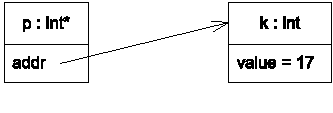
\includegraphics{BasicCPP/Figures/Pointer.pdf}
    \end{center}  
    \caption{A value of a pointer to an int (int*) is the adress of a memory location which
              has the size and is interpreted as an integer.
             \label{figPointer}} 
  \end{figure}
%\end{latexonly}  

%\begin{htmlonly}
%  \begin{rawhtml}
%    <center>
%      <img src="BasicCPP/Figures/Pointer.gif">
%    </center>
%    <br>
%    <center>
%        A value of a pointer to an int (int*) is the adress of a memory location which
%              has the size and is interpreted as an integer.
%    </center>
%  \end{rawhtml}  
%  \begin{figure}\label{figPointer}\end{figure}
%  \vspace{5mm}
%\end{htmlonly}  

Pointers a simply addresses in memory. They are used extensively
in C and C++ and a thorough understanding of pointers is
essential for good programming skills. Typically pointers
in C++ are typed, i.e.\ they point to a memory location which
contains a certain specified data type. For example, in the following
listing we define a pointer \verb+p+ to an integer and an
integer variable \verb+k+.
{\small \begin{verbatim}
int* p;                 // Defining a pointer to a 2 byte
                        //   (sizeof(int)) memory location.
int k = 17;             // Defining an integer variable.

p = &k;                 // Pointer p now points to address of k.

cout << p;              // Writes the address of p.

cout << (*p);           // Pushes 17 onto the output stream
                        //   (the pointer p is dereferenced).
\end{verbatim}}
\noindent
We then use the address operator \verb+&+ to set the pointer \verb+p+
to the address of \verb+k+.
The result is graphically depicted in figure \ref{figPointer}.
We can \index{address!of a variable}
either print the contents of the pointer variable itself which
will be an address or we can dereference the pointer, using the
dereferencing operator \verb+*+. The result of the dereferencing
\index{pointers!dereferencing}
operation is the contents of the memory position to which
the pointer \verb+p+ points.

%------------------------------------------------------------------------

\subsection{The NULL pointer}

Commonly a NULL pointer is used when the address to which the
\index{pointers!\verb+NULL+ pointer}
pointer should point is not yet determined (NULL implies undefined).
{\small \begin{verbatim}
T* p = NULL;
\end{verbatim}}
\noindent
Here we defined a pointer to data type \verb+T+ and initialized
it to the NULL-pointer. It is good programing practice to initialize all
pointers which do not yet point to valid memory locations to the NULL
pointer.

%----------------------------------------------------------------------

\subsection{Pointers and strong typing}

Similarly, if we want to keep the data type to which the pointer
points unspecified we can use a \verb+void*+. ANSI C allows pointer
\index{pointers!\verb+void+ pointer}
of type \verb+void*+ to be assigned to any pointer and also any
pointer to be assigned to \verb+void*+. In C++ we can still assign
a pointer of any type to \verb+void*+, but if we want to assign
a \verb+void*+ to any other pointer type we must make an explicit
\index{pointers!type casting}
type casting. This is illustrated in the following listing
{\small \begin{verbatim}
void* pvoid;
char* str;

pvoid = str;            // quite legal in C++
str = pvoid;            // illegal in C++
str = (char*)pvoid      // legal with type-casting
\end{verbatim}}

%------------------------------------------------------------------------

\subsection{Constant pointers and pointers to constants}

In C++ one can declare either the pointer itself constant (i.e.\ the memory
location it points to may not change), or the item it points to as constant
or both. This is illustrated in the following demostration code:
{\small \begin{verbatim}
int k=17, l=5;

      int*       ip   = &k;
const int*       cip  = &k;
      int* const ipc  = &k;
const int* const cipc = &k;

   ip = &l;     //     legal, pointer value may change.
  *ip = 32;     //     legal, what ip points to may change.

  cip = &l;     //     legal, pointer value may change.
 *cip = 32;     // not legal, what cip points to may not change.

  ipc = &l;     // not legal, pointer value may not change.
 *ips = 32;     //     legal, what ipc points to may change.

 cipc = &l;     // not legal, pointer value may not change.
*cips = 32;     // not legal, what cipc points to may not change.
\end{verbatim}}

%------------------------------------------------------------------------

\subsection{Pointer arithmetic}

Pointer arithmetic calculates memory addresses. One can increment, decrement,
add an integer to a pointer, subtract an integer from a pointer or subtract
one pointer from another pointer.

Pointers in C++ are generally typed. For example, a \verb+double*+ points
to a memory location of the size of a double precision variable. Adding an
integer \verb+n+ to the pointer adds \verb+n+ times the size of the data
type it points to to the address it points to.
{\small \begin{verbatim}
int *ip = new int[10];

int* ip2 = ip = ip+2;

cout << " ip2 = " <<  ip2 << endl;  // prints address of ip[2];
cout << "*ip2 = " << *ip2 << endl;  // print ip[2];
\end{verbatim}}

Similarly we can subtract a pointer, increment a pointer (adding 1 times the
size of its data type to the address it points to) and decrement a pointer.
Subtracting two pointers of the same type from one another returns the distance
in memory between the two pointers in multiples of the size of the data type
they point to.

%---------------------------------------------------------------------

\subsection{Pointers to functions: passing a function as a function argument}

For science and engineering applications it is quite common that one wants to
pass a function to another function as an argument. Functions in C++ are
passed as a and executed from a pointer. For example
{\small \begin{verbatim}
double (*f)(const double&)
\end{verbatim}}
\noindent
defines a pointer variable \verb+f+ of type function-pointer. We can assign
this function pointer to any function which is type-compatible with the
above signature. Consider the following listing:
{\small \begin{verbatim}
#include <iostream.h>
#include <math.h>

double sqr (double x)
{return x*x;}

void main()
{
  double x = 1.7;
  double (*f)(double) = NULL;
  f = sin;
  cout << "sin(x) = " << f(x) << endl;
  f = sqr;
  cout << "sqr(x) = " << f(x) << endl;
}
\end{verbatim}}
\noindent
We declare and initialize a double precision variable \verb+x+ and a pointer variable
\verb+f+ which points to a function which receives a \verb+double+ as argument and
returns a \verb+double+. We first assign \verb+f+ to the function \verb+sin+ defined
in the standard C++ library \verb+math.h+. Calling \verb+f(x)+ returns \verb+sin(x)+.
We then assign the function pointer \verb+f+ to our own function \verb+sqr+. Now
\verb+f(x)+ returns \verb+x*x+.

In a similar way we pass a fuction to another function as an argument. Consider, for
example, that you want to write a numerical integration routine which evaluates the
integral of any given function between given integration boundaries. In other
words,we want to evaluate
\begin{equation}
  I = \int_a^b f(x) dx \nonumber
\end{equation}
for any given $f(x)$, $a$ and $b$. The function header could look like this:
{\small \begin{verbatim}
double Integrate (double (*func)(double), const double a,
                  const double b, const double eps);
\end{verbatim}}
\noindent
where \verb+eps+ is the accuracy with which we want to approximate the exact integral.

A simple, yet quite robust integration rule is Simpson's integration rule:
\begin{eqnarray}
  I & \approx & \frac{h}{3} [f(a)+f(b)+4(f(a+h) + f(a+3h) + \dots + f(b-h))
       \nonumber \\
    &  & + 2(f(a+2h)+f(a+4h)+ \dots +f(b-2h))] \nonumber
\end{eqnarray}
Here $h$ is the stepsize on which the function is evaluated, i.e.\ the integration
interval $[a,b]$ is subdevided into $N$ equally sized subintervals with width
\begin{eqnarray}
  h = \frac{b-1}{N} \nonumber
\end{eqnarray}
Below we give a simple implementation of the Simpson integration rule:

\noindent{\small\input{BasicCPP/Programs/Simpson.cpp}}

If we run the example program which integrates $e^x$ with 100 intervals integrating
over the range $[0,1]$, we obtain the following result:

\noindent{\small\begin{verbatim}
Enter no of intervals = 40
Enter integration range a b : 0 1
Simpson: 1.46265
\end{verbatim}}

%------------------------------------------------------------------------

\section{Arrays}
An array \index{array} is a contiguous region of storage, large enough to hold all
its elements. The array elements are thus ordered in memory and can be accessed via
numeric subscripts.

\subsection{Arrays in static memory}

We can declare an array of a fixed size by using the element access operator \verb+[]+.
For example,  \verb+int iArray[5]+ reserves a memory for 5 integer variables which are
\index{array}
accessed via \verb+iArray[0]+, \dots, \verb+iArray[4]+. Arrays can be multi-dimensional.
For example, in the listing below we define a (3x3) array \verb+M+ of double precision
variables.
\index{array!multi dimensional} The elements are accessed via
\verb+M[i][j]+ where \verb+i+ and \verb+j+ run from 0 to 2. The function
\verb+sizeof(M)+ \index{\verb+sizeof+} returns the size of the entire memory
block of 9 double precision
floating point numbers. Note that \verb+nrows+ and \verb+ncols+ are defined as
constants. This is essential, because the size of an array in static memory must
be known at compile time.

\noindent {\small \input{BasicCPP/Programs/StaticArray.cpp}}

An array can also be declared and initialized in a single statement.
\index{array!declare and initialize} For example
{\small \begin{verbatim}
int intArray[] = {1, 78, 12, 5};
\end{verbatim}}
\noindent
allocates memory for 4 integer variables, initializes these memory positions the
relevant integer values and sets the pointer \verb+intArray+ to the start of that memory
block. \index{array!declare and initialize}
Similarly
{\small \begin{verbatim}
double matrix[3][3] = { {1.0, 1.7, 2.3},
                        {3.2, 7.9, 0.4},
                        {0.1, 9.9, 4.2} };
\end{verbatim}}
\noindent
declares and initializes a 3x3 array o floating point variables.
\index{array!declare and initialize}
while
{\small \begin{verbatim}
double matrix[3][3] = { {1.0},
                        {3.2},
                        {0.1} };
\end{verbatim}}
\noindent
declares a 3x3 array and initializes the first column. Note that unlike FORTRAN,
C++ stores its arrays in row-major order.

%-----------------------------------------------------------------------------------

\subsection{Arrays in dynamic memory}

Static allocation of arrays has, however, a few severe disadvantages. If one, for example,
writes a function for least squares fitting of a set of data points to a function, the
number of data points are mot generally known beforehand. One could make the assumption
that the user will never use more than say 200 data points. Then the user could never
supply more than 200 data points. Furthermore, if he supplies only 5 data points the program
would still use memory for 200 points. Finally, the meory cannot be released while the
array is in scope, even if it is no longer needed.

An alternative approach is to reserve memory at run-time. This is done in $C^{++}$ via
the \verb+new+ operator. If we want to reserve memory for an array of \verb+n+ integer
variables we can do this by
{\small \begin{verbatim}
int *vector = new int[n];
\end{verbatim}}
\noindent
This statement declares an integer pointer \verb+vector+, reserves a block of
contiguous memory space, large enough for \verb+n+ integer variables, and sets
the address of the pointer variable \verb+vector+ to the start of the memory block.
The representation in memory is illustrated in figure \ref{figDynamicArray1D} 
(we replaced the
name of the pointer variable by \verb+v+ to achieve a more compact notation).


%\begin{latexonly}
  \begin{figure}[htb]
    \begin{center}  
      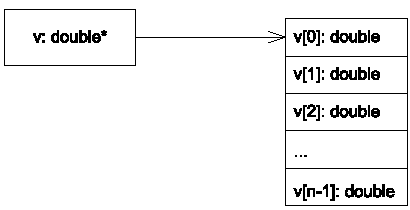
\includegraphics{BasicCPP/Figures/DynamicArray1D.pdf}
    \end{center}  
    \caption{Memory structure for a one-dimensional dynamic array.
             \label{figDynamicArray1D}} 
  \end{figure}
%\end{latexonly}  

%\begin{htmlonly}
%  \begin{rawhtml}
%    <center>
%      <img src="BasicCPP/Figures/DynamicArray1D.gif">
%    </center>
%    <br>
%    <center>
%        Memory structure for a one-dimensional dynamic array.
%    </center>
%  \end{rawhtml}  
%  \begin{figure}\label{figDynamicArray1D}\end{figure}
%  \vspace{5mm}
%\end{htmlonly}  

Note that \verb+n+ need not be constant and can be read in from the terminal. When we
no longer require the vector we can free the memory and thereby conserve our
hardware resources. This is done by the following statement
{\small \begin{verbatim}
delete[] vector;
\end{verbatim}}

The following program shows how one could dynamically allocate a two-dimensional
array (which can be used to represent the data of a matrix).

\noindent {\small \input{BasicCPP/Programs/DynamicArray.cpp}}

An example output of the program is shown below:

\noindent{\small \begin{verbatim} 
Enter number of rows : 2
Enter number of columns : 3
Now enter the elements of the (2x3) matrix M :
M[1,1] = 1
M[1,2] = 2
M[1,3] = 3
M[2,1] = 2
M[2,2] = 3
M[2,3] = 1
sizeof(M)    = 4
sizeof(M[1]) = 4
sizeof(M[1][1]) = 8
\end{verbatim}}

\verb+M+ is defined as a pointer \index{pointers} to a pointer to a double precision variable.
\index{array!dynamic memory} \index{\verb+new+} \index{\verb+delete+}
\index{memory!dynamic} \index{matrix!dynamic memory}
We first reserve memory for \verb+nrows+ pointers and set the pointer \verb+M+ to the
start of that memory block. For each of the \verb+nrows+ pointers we reserve
enough memory for \verb+ncols+ double precision variables. The memory arrangement
is illustrated in figure \ref{figDynamicArray2D}.

%\begin{latexonly}
  \begin{figure}[htb]
    \begin{center}  
      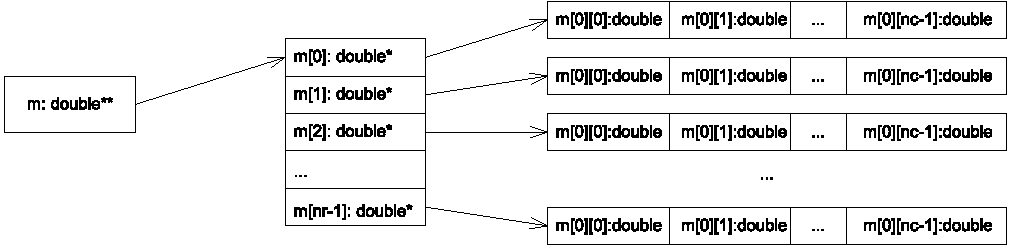
\includegraphics{BasicCPP/Figures/DynamicArray2D.pdf}
    \end{center}  
    \caption{Memory structure for a two-dimensional dynamic array.
             \label{figDynamicArray2D}} 
  \end{figure}
%\end{latexonly}  

%\begin{htmlonly}
%  \begin{rawhtml}
%    <center>
%      <img src="BasicCPP/Figures/DynamicArray2D.gif">
%    </center>
%    <br>
%    <center>
%        Memory structure for a two-dimensional dynamic array.
%    </center>
%  \end{rawhtml}  
%  \begin{figure}\label{figDynamicArray2D}\end{figure}
%  \vspace{5mm}
%\end{htmlonly}  

Note that \verb+sizeof(M)+ and \verb+sizeof(M[1])+ both return the memory required
for a pointer variable while \verb+sizeof(M[1][1])+ returns the memory required for
a double precision variable. \index{\verb+sizeof+}

When using dynamic memory allocation, one should be careful that there are no
\index{memory!dynamic} \index{pointers!null-pointer}
memory leaks (i.e.\ that all memory which is allocated during run-time is
deallocated again --- preferably as soon as it is no longer required) and that
the integrity of pointers is ensured (i.e.\ that pointers do not end up pointing to
memory areas which are reserved for other purposes). It is a good programming
practice to set all pointers for which there is no memory reserved equal to NULL
\index{\verb+NULL+} (known as the null pointer).

%----------------------------------------------------------------------

\subsubsection{Example program: Linear regression}

We demonstrate the usefulness of dynamic memory with a general linear regression
\index{examples!linear regression}
program. In this case an experimentalist has measured a set of data points and he
wants to fit the ``best'' straight line through these data points.

Consider a set of data points $\{(x_i,y_i), \; i=1 \dots n\}$.
By minimizing the sum of the squares of the error (least-squares fit) one obtains the
following expressions for the slope of the straight line and its $y$-intercept:
\begin{eqnarray}
  \mbox{slope} &=& \frac{\left( \sum_{i=1}^n x_i \right) \cdot \left( \sum_{i=1}^n y_i \right)
                      - n \sum_{i=1}^n x_i y_i }
                        {\left( \sum_{i=1}^n x_i \right)^2
                      - n \sum_{i=1}^n x_i^2 } \nonumber \\
  y-\mbox{intercept} &=& \frac{ \sum_{i=1}^n y_i - \mbox{slope} \cdot \sum_{i=1}^n x_i}
                                {n}  \nonumber
  \label{linearregression}
\end{eqnarray}

The following little program will ask for the number of data points and it
will determine the best straight-line fit to these points:

\noindent {\small \input{BasicCPP/Programs/LinearRegression.cpp}}

Note that we declare the pointer variables in the main program and that we reserve memory
for the arrays and assign the pointer variables to the starting address of these arrays
in the function \verb+readDataPoints+. We thus have to pass the pointers by reference.
Note also that \verb+double* x+ and \verb+double x[]+ are type compatible. Once we now
longer require the arrays, the memory is released via the array-delete operator,
\verb+delete[]+.

As an example we ran the program with the five data points indicated by asterisks in
figure \ref{linear} and have plotted the linear regression result onto the same figure.
\index{examples!linear regression}

\begin{figure}[htb]
  \begin{center}
    \input{BasicCPP/Figures/Linear.pic}
  \end{center}
  \caption{Linear regression result. \label{linear}}
\end{figure}

%---------------------------------------------------------------------------------

\subsection{Array versus vectors and matrices}

We will differentiate between C and C++ arrays (static or dynamic) and vectors
and matrices. Arrays can represent the data structure of a vector or a matrix,
but vectors and matrices have associated with them certain operations like
the vector addition or the vector dot product or matrix multiplication. Also,
when using C-type arrays (via pointers) there is no automatic range checking.

Later in this book we shall discuss array and vector and matrix classes which do
support controlled element access and data-type specific functionality. This will
allow us to write code which is very similar to Matlab or Mathematica code in
that we will be able to, for example, directly multiply matrices in very simple
and very powerful code like the code extract shown below:
{\small \begin{verbatim}
matrix<double> A(n,n), B(n,n), C(n,n)
A = B*C;
cout << "matrix B x matrix C = " << A;
\end{verbatim}}

%------------------------------------------------------------------------

\subsection{Character arrays as strings}

C++ has no predefined string data type. Instead one uses arrays to
\index{arrays!of \verb+char+} \index{strings} characters, which behave
many, but not in all ways identical to any other array type. There are,
however, some important differences which are illustrated in the following
code:
{\small \begin{verbatim}
#include <iostream.h>

void main()
{
  char str[20] = "This is a string";
  char* pchar = str;
  cout << str    << endl;         // prints "This is a string"
  cout << pchar << endl;          // prints "This is a string"

  int ivec[5] = {1, 2, 3, 4, 5};
  int* pvec = ivec;
  cout << pvec << endl;           // prints the address of ivec[0]
  cout << (*pvec) << endl;        // prints its contents, 1

  ++ pvec;
  cout << (*pvec) << endl         // prints the second element, 2
}
\end{verbatim}}
\noindent
In the above listing, both \verb+str+ and \verb+p+ are effectively
pointers to characters. The first statement does a lot of things
in the background. It first defines \verb+str+ as
a pointer to \verb+char+, reserves 20 bytes (for 19 characters
\index{memory!allocation of}
and the terminating \verb+\0+ character) in memory, initializes these
memory positions with the string characters and the terminating NULL
character and finally it sets the pointer \verb+str+ to the starting position
of this memory area. The second statement simply defines a pointer
\verb+pchar+ to \verb+char+ and initializes this pointer to the memory position
\index{pointers!assignment}
of \verb+str+. Pushing \verb+pchar+ onto the output stream
prints not only the first character \verb+'T'+, but the entire string.
\index{pointers!of \verb+char+!pushing on output stream}
This behavior is not usual for pointers. In fact, it only works like
this for pointers to the data type \verb+char+. The reason for this
is historical -- it simulates some functionality of a string data type.
\index{strings!pushing on output stream}
If we do the same
for an array of integers then things look quite differently. We
first define a vector of 5 integers which are initialized to 1--5.
We then define a pointer \verb+pvec+ and set it to the starting
address of this vector. Now printing out \verb+pvec+ results
\index{pointers!pushing on output stream}
in the more standard behavior, i.e.\ the address of the first element
of the vector is printed. Dereferencing the pointer results in the
\index{pointers!dereferencing}
contents of this memory position which is the first element in the
array. Since the vector is typed (of type \verb+int*+) we can
increment the vector using the standard pre- or post-fix incrementation
\index{pointers!incrementing} \index{pointers!decrementing}
operator. The result is that the pointer now points to the next memory
area of size \verb+sizeof(int)+ and dereferencing the pointer now
yields the second element of the vector.

Since $C^{++}$ supports most aspects of $C$ one can define a string on a
\verb+char+-pointer and use the ANSI-$C$ string manipulation functions like
\verb+strcpy+ for string copy, \verb+strcat+ for string concatenation,
\verb+strcmp+ for string comparison and so forth.

Note that strings are really data types with their own functionality (e.g.\ addition
would imply string concatenation). It is hence usually a good idea to either
write your own string class or to use a string class supplied with your compiler
or by an independant vendor.

%================================================================

\section{Function templates}
\index{\verb+template+!function templates}

Templates are the way in which C++ implements generic functions.
Traditionally, if you define a function \index{functions} you would have
to define it for every data type with which you would want to be able to call that
function. If you would write a mathematical library containing Bessel functions
you would have to define the Bessel functions for \verb+int+, \verb+float+,
\verb+double+, \verb+long double+ and \verb+complex+.
If you want to improve your algorithm at a later stage you would have to search
for all definitions of the Bessel function and make the relevant changes.
This is cumbersome and prone to errors. Similarly, you would typically have to
write a Simpson integrator function for functions of type \verb+float+, \verb+double+
and \verb+long double+ and possibly also for your own data types like, for example,
\verb+Rational+. By defining the Simpson integrator on a template
\index{\verb+template+}
{\small \begin{verbatim}
template <class T>
T Simpson (T (*f)(const T&), const T& a, const T& b, const int nintvl);
\end{verbatim}}
\noindent
the compiler will automatically generate the code for the data types required
in the code. The phrase  \verb+ template <class T> + in front of the function
\index{\verb+template+} definition specifies that the function is defined on a
template. Here \verb+T+ is a type-variable (you can use your own variable name,
if you like. At least one of the arguments of the function must refer to type \verb+T+.
\index{arguments!for templates} Since the return value of a function does not
participate in defining a unique signature (since the user need not use the return value), it
is not sufficient that the template type is referred to only in the return value of the
function.

Now, if you call \verb+Simpson+ twice, once with a function
of the form
{\small \begin{verbatim}
double func(const double& x);
\end{verbatim}}
\noindent
and once with a function of the form
{\small \begin{verbatim}
Rational fr(const Rational& r)
\end{verbatim}}
\noindent
then the compiler will write for you two functions, one with every occurance of
\verb+T+ replaced by \verb+double+ and one with every occurance of \verb+T+
replaced by \verb+Rational+.

It is interesting to note that the template argument \verb+T+ can refer to object types,
function names, constant expressions or character strings.

\subsection{Example program: Bubble-sort}
\index{examples!bubble sort} \index{sorting algorithms!bubble sort}

We illustrate function templates via a simple bubble-sort program. Since the
program will be defined on a template, it will be able to sort arrays of any
data type, as long as there is a greater-as operator, \verb+>+, and an assignment
operator, \verb+=+, defined for the data type (or the class). In
\index{vector}
our example program we sort an array of \verb+float+ and an array of \verb+char+
with the same Bubble sort routine.

\noindent {\small \input{BasicCPP/Programs/BubbleSort.cpp}}

The applicability of this sorting routine is, however, not limited to predefined
data types. It can also be used for user defined data types (e.g. an array of
\index{data types!user defined}
rational numbers or an array of employee records).

%------------------------------------------------------------------------

\subsection{Multiple templates}

We can also define a function (or a class) on multiple templates. For example,
you might want to sort an associative array (also called a dictionary or a map).
An associative array keeps for each element a key. Given the key, we can access
the value (this is an abstraction of accessing the array elements via integers).

A simple, non-object-oriented way of defining a sorting algorithm for an associative
array would be to use two template types:
{\small \begin{verbatim}
template <class K, class V>
void quickSort (K keys[], V values[], const int length);
\end{verbatim}}

%------------------------------------------------------------------------

\subsection{Overloading template functions}
\index{overloading!functions}\index{functions!overloading}

Template functions can be overloaded just like any other function.
Consider, for example, the following program listing

\noindent {\small \input{BasicCPP/Programs/Maximum.cpp}}

The output of the above program is shown below:

\noindent{\small\begin{verbatim}
a, b = 5.1, 1.23
Max(a,b) = 5.1

v = [9, 2, 11, 7, 8]
Max(v,4) = 11
\end{verbatim}}

\noindent
Here we defined two version of the function \verb+Max+. Both
versions are defined on a template.
\index{\verb+template+!function templates}
The first version takes two scalar arguments (for example
two floating point numbers) and returns the larger of the
two. The second version, which carries the same name as
the first takes, a pointer variable (for an array) as the
first argument and an integer argument specifying the number
of elemnts in the array. This function returns the largest
of the array elements.
Note that the first argument, \verb+vec+, is defined as
{\small \begin{verbatim}
const T* const vec
\end{verbatim}}
\noindent
In this case both, the pointer variable \verb+vec+, and the
\index{pointers!\verb+const+}
memory locations it points to (the array elements) are treated
\index{arrays!const} as \verb+const+.

%------------------------------------------------------------------------

\section{Recursion}

Recursion occurs when a function calls itself, either directly or indirectly.
Many mathematical problems can be defined very elagently using recursion.
We have direct recursion when a function calls itself. Indirect recursion involves,
for example, a function \verb+f1+ calling another function \verb+f2+ which calls again
\verb+f1+. For example the right-hand side calling hierarchy in figure
\ref{figRecFuncs} contains both direct (\verb+f2+ calling itself) and indirect recursion
(for example, \verb+f6+ calls \verb+f8+ calls \verb+f9+).

Often one finds simple functions, like the factorial function, implemented recursively:
{\small \begin{verbatim}
long int factorial(const long int n)
{
  long int local = n;
  if (n>=2)
    local *= factorial(n-1);
  return local;
}
\end{verbatim}}
\noindent
Note, however, that if we calculate $n!$ the function, \verb+factorial+, is called $n \!\! - \!\! 1$
times and hence $n \!\! - \!\! 1$ stack frames are created, each frame containing a copy of the
local variable \verb+local+, the function argument \verb+n+ and the calling address.
Finally the stack has to be unwound before the final result is passed to the function calling
\verb+factorial+. A good proportion of these overheads is avoided by mapping the recursive
algorithm onto a non-recursive one:
{\small \begin{verbatim}
long int factorial(const long int n)
{
  long int local = n;

  for (int i=n-1; i>=2; i--)
    local *= i;

  return local;
}
\end{verbatim}}

Furthermore, recursive cycles in a function calling diagram complicate the analysis, design and testing
significantly. In Figure \ref{figRecFuncs} a function calling lattice (a lattice is a tree for which
branches can share descendents) is compared to a function calling diagram which contains
direct and indirect recursion. The lattice structure is not only simpler to comprehend, but it
has the additional advantage that the leaves of the tree (f6, f9 and f10) can be tested
independetly, and once it is established that these work correctly, the next level of functions
can be tested. These functions (f5,f7 and f8) call only functions which have been tested already.
On the other hand, if the function diagram contains indirect recursion (f4--f6 and f6--f8--f9), then
the function making up the recursive cycle cannot be tested independetly.


%\begin{latexonly}
  \begin{figure}[htb]
    \begin{center}  
      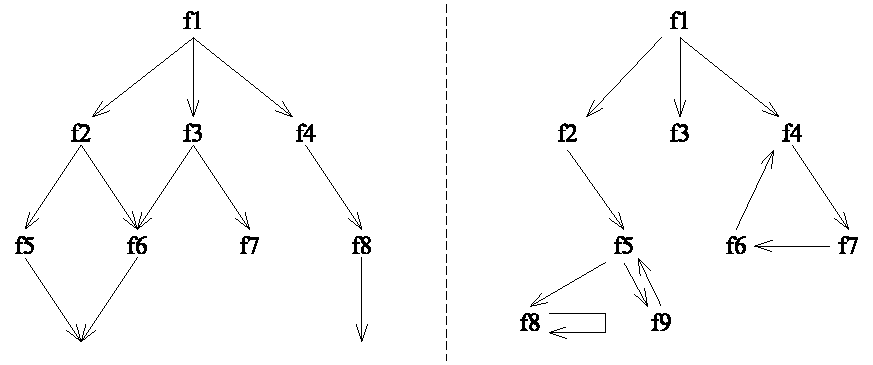
\includegraphics{BasicCPP/Figures/Recursion.pdf}
    \end{center}  
    \caption{A lattice function calling hierarchy (left) compared to a more
              general function calling diagram containing direct and indirect
              recursion. 
             \label{figRecursion}} 
  \end{figure}
%\end{latexonly}  

%\begin{htmlonly}
%  \begin{rawhtml}
%    <center>
%      <img src="BasicCPP/Figures/Recursion.gif">
%    </center>
%    <br>
%    <center>
%        A lattice function calling hierarchy (left) compared to a more
%              general function calling diagram containing direct and indirect
%              recursion.
%    </center>
%  \end{rawhtml}  
%  \begin{figure}\label{figRecursion}\end{figure}
%  \vspace{5mm}
%\end{htmlonly}  

Hence, both direct and indirect recursion havesignificant disadvantages and it is generally a
good idea to try and map recursive dependancy cycles onto lattice structures. This may, of
course not always be a reasonable option.

%------------------------------------------------------------------------

\section{Simple file I/O and simple strings}
\index{file!input/output} \index{strings}

The following program illustrates simple file input and output as well as simple
strings. As is the case for vectors and matrices, strings in $C^{++}$ are best
handled by defining for them an abstract data type (a class). \index{abstract data type}
\index{\verb+class+!string}
This will be done in the coming chapters. Here we use the standard $C^{++}$ strings
which are defined as arrays of characters with a terminating \verb+NULL+ character
(\verb+\0+). \index{array!of char} \index{\verb+NULL+ character}
Hence the string variable \verb+inputfilename+ is defined as an array of
60 characters (the string can be no longer than that length with the actual length
determined by the position of the \verb+NULL+ character in that array of characters).
\index{strings!null terminated}
The function \verb+strlen()+ \index{\verb+strlen()+ function} returns the length of
the string by determining the position of the \verb+NULL+ character.

A string can also be declared and initialized in a single statement
{\small \begin{verbatim}
  char* myname = "Peter Smith";
\end{verbatim}}
\noindent
In this case the compiler allocates enough memory to hold the relevant string
(including the terminating \verb+'/0'+-character)
\index{strings} \index{memory!dynamic allocation of}
and sets the pointer \index{pointer!string} to the start of that memory space.

\subsection{Example program: Replacing all occurances of a string in a file}

\noindent {\small \input{BasicCPP/Programs/Replace.cpp}}
\noindent
An input file is opened by creating an object of class \verb+ifstream+
\index{input-file stream} with
\index{file!input/output} \index{file!opening} \index{file!closing}
\index{\verb+ifstream+} \index{file!name}
the file name as parameter. The statement
{\small \begin{verbatim}
if (!infile) ...
\end{verbatim}}
\noindent
checks whether the file \verb+infile+ was opened successfully. We use the stream
method \verb+get()+ instead of the \verb+>>+ operator, since the latter
\index{\verb+get()+ stream method} \index{\verb+>>+ operator}
filters out spaces, carriage return and line feed characters.
When the files are no longer required they are closed via the stream method
\verb+close()+. \index{file!closing}

When running the program on its own source code, replacing \verb+oldStr+, we
obtain the following output:

\noindent{\small\begin{verbatim}
Enter name of input file: Replace.cpp
Enter name of output file: Replace.out
Enter string to be replaced throughout file: oldStr
Enter replacement string: THE_VERY_OLD_STRING
The string <oldStr> has been replaced by <THE_VERY_OLD_STRING> 8 times.
\end{verbatim}}

%------------------------------------------------------------------------

\section{Constants and inline functions instead of macros}

For $C$-programmers it was common to define constants \index{constants} via the
macros \index{macros} \index{\verb+#define+ directive}. For example, one would define
{\small \begin{verbatim}
#define eps 1.0e-8
\end{verbatim}}

\noindent
In this case the $C$ or $C^{++}$ preprocessor \index{preprocessor} replaces every
occurance of \verb+eps+ with \verb+1.0e-8+ before the source code is forwarded to
the compiler. This has several disadvantages. Firstly any compiler error involving
\verb+eps+ will refer to \verb+1.0e-8+ and not to \verb+eps+.
If the code is long it might take the programmer a very long time
before he finds the error. The same problem is encountered when one uses a symbolic
debugger, since \verb+eps+ is never entered into the programs symbol table.
Furthermore, the constant \verb+eps+ cannot be given an explicit type.

All these problems can be solved in $C^{++}$ by replacing the above macro by
\index{macros}
{\small \begin{verbatim}
const double 1.0e-8
\end{verbatim}}
\index{\verb+const+}
\noindent
The constant can be defined either locally or globally (preferably locally).

An even bigger sin is to use macros \index{macros} in order to define inline functions.
\index{functions!inline} \index{inline} Consider the following commonly used macro
{\small \begin{verbatim}
#define SQR(x) x*x
#define MAX(x,y) ((x) > (y) ? (x) : (y))
\end{verbatim}}

\noindent
One needs the parenthesis around \verb+x+ and \verb+y+ in order to allow the user
to use the macro with expressions. The macros look harmless enough. Consider,
however, the following pitfalls:
{\small \begin{verbatim}
y = SQR(1+2);     // result: 5 instead of 9
z = MAX(x++,y);
\end{verbatim}}
\noindent
In the first case the macro expansion results in \index{macros}
{\small \begin{verbatim}
y = 1+2 * 1+2;
\end{verbatim}}
\noindent
which evaluates to 5 (since multiplication has higher precedence than addition).
In the second case \verb+x+ will be incremented either once or twice, depending
on whether \verb&(x+1)& is greater than \verb+y+ or not. It should be clear that
macros like the above are not only bad style but downright dangerous. Again there
is an elegant alternative available in $C^{++}$:

\noindent {\small \input{BasicCPP/Programs/NoMacro.cpp}}

\index{functions!inline} \index{\verb+inline+}
\index{\verb+template+!function templates}

The output of the program is:

\noindent{\small \begin{verbatim}
sqr(2+1) = 9
max(a,b) = 2.1
\end{verbatim}}

\noindent
Declaring these functions as \verb+inline+ \index{\verb+inline+} avoids the function
call overheads.
Note, however, that \verb+inline+ is a request to the compiler which might be
ignored if the compiler feels it is not a good idea (e.g.\ for example for recursive
functions and complex functions).

Defining the functions on a template
\index{\verb+template+!function templates}  ensures that \verb+sqr+
and \verb+max+ can be used for several data types (e.g.\ for integers,
floating point numbers, or your own classes --- say a class of rational numbers).
In contrast to the  macro \index{macros} definitions, the inline functions
\index{functions!inline} are type-safe.

%--------------------------------------------------------------------

%%\section{Building non-object-oriented libraries in C++}

%--------------------------------------------------------------------

\begin{exercises}
  \item The rules for leap years are a little convoluted: every 4'th year is
        a leap year except every century which isn't except every 4'th century 
        which is.
         Write a function \verb+leapyear+ which takes an integer as argument
          and returns 1 if its is a leap year and zero otherwise. In you main program,
          read in years in a loop until the user enters a zero for the year. For
          each year enetered, the program should report whether it is a leap
          year or not. (Hint: use
          the remainder operator \verb+%+ in your leap year function).
  \item Write a program which reads in the parameters $a$, $b$ and $c$
          of a parabola $y(x) \! = \! ax^2+bx+c$ and gives as output the roots
          of the parabola as well as its turning point. The roots of a parabola
          are given by
          \begin{eqnarray}
             x_{1,2} = \frac{-b \pm \sqrt{b^2 - 4ac}}{2a}
          \nonumber \end{eqnarray}
          and its turning point is given by
          \begin{eqnarray}
            x_0 = - \frac{b}{2a}; \hspace{8mm} y_0 = y(x_0)
          \end{eqnarray}
          (there is a \verb+sqrt+ function in the standard C++ library {\bf math.h}).
  \item Write a program which reads in a series of floating point numbers
         (use dynamic memory allocation), calculates their mean and their
         \index{memory!dynamic allocation of}
         standard deviation from that mean (declare functions
         \verb+mean+ and \verb+stddeviation+).
         \index{examples!statistical mean}
         \index{examples!standard deviation}
         The mean and the standard deviation are defined as follows:
         \begin{eqnarray}
            \mbox{mean}        &=& \frac{1}{N} \sum_{i=1}^N x_i \nonumber \\
            \mbox{stddeviation} &=& = \sqrt{\sum_{i=1}^N (x_i - \mbox{mean})^2}
                \nonumber
         \end{eqnarray}
  \item Write a program which reads in a string \index{strings} of up to 80
         characters and which gives as output the upper case version of that
         string together with the number of characters in that string. For the
         case where the input string is upper case already, let it print
         a message to that effect.
         (The standard $C$ functions \verb+int toupper(int chr)+ and
         \index{\verb+toupper()+!convert to upper case}
         \index{\verb+isupper()+!check if upper case}
         \verb+int isupper(int chr)+  are defined
         in the library \verb+<ctype.h>+. \index{\verb+<ctype.h>+}
         \verb+isupper+ returns nonzero if \verb+chr+ is an upper case
         character (\verb+A+ to \verb+Z+).
  \item Write a procedure \verb+swap+ which swaps any two objects \verb+x+ and
         \verb+y+ (Hint: use function templates).
         \index{swap function} \index{\verb+template+!function templates}
         Write a short main program which illustrates how this procedure can be
         used to swap two floating point numbers, two characters, two strings
         and two arrays of floating point numbers (declare any two strings
         and arrays). Explain what happens in the latter two cases (what
         happens to the pointer variables and to the memory they point to?).
  \item Write a program which reads the source code of a $C^{++}$
          program and removes all the comments from it.
  \item Write a series of functions calculating the circumference of various
           geometrical shapes. Each of the functions should be called
           \verb+circumference+ (function overloading).
          If it is called with a single parameter it is to assume
          that the shape whose circumference you want to calculate
          is a circle and the parameter is the radius. If you call it with
          two parameters it should assume that the shape is a rectangular
          with the two parameters being the width and height of the
          rectangular. If you call it with 3 parameters it should assume
          the shape is a triangle with the parameters being the three
          side lengths.
\end{exercises}
